%==================== CHAPTER 4 ====================
\ChapterPage{Design Of the System}

\section{System architecture}

\subsection{Data Flow Diagrams}

\begin{bodyfigure}[H]
  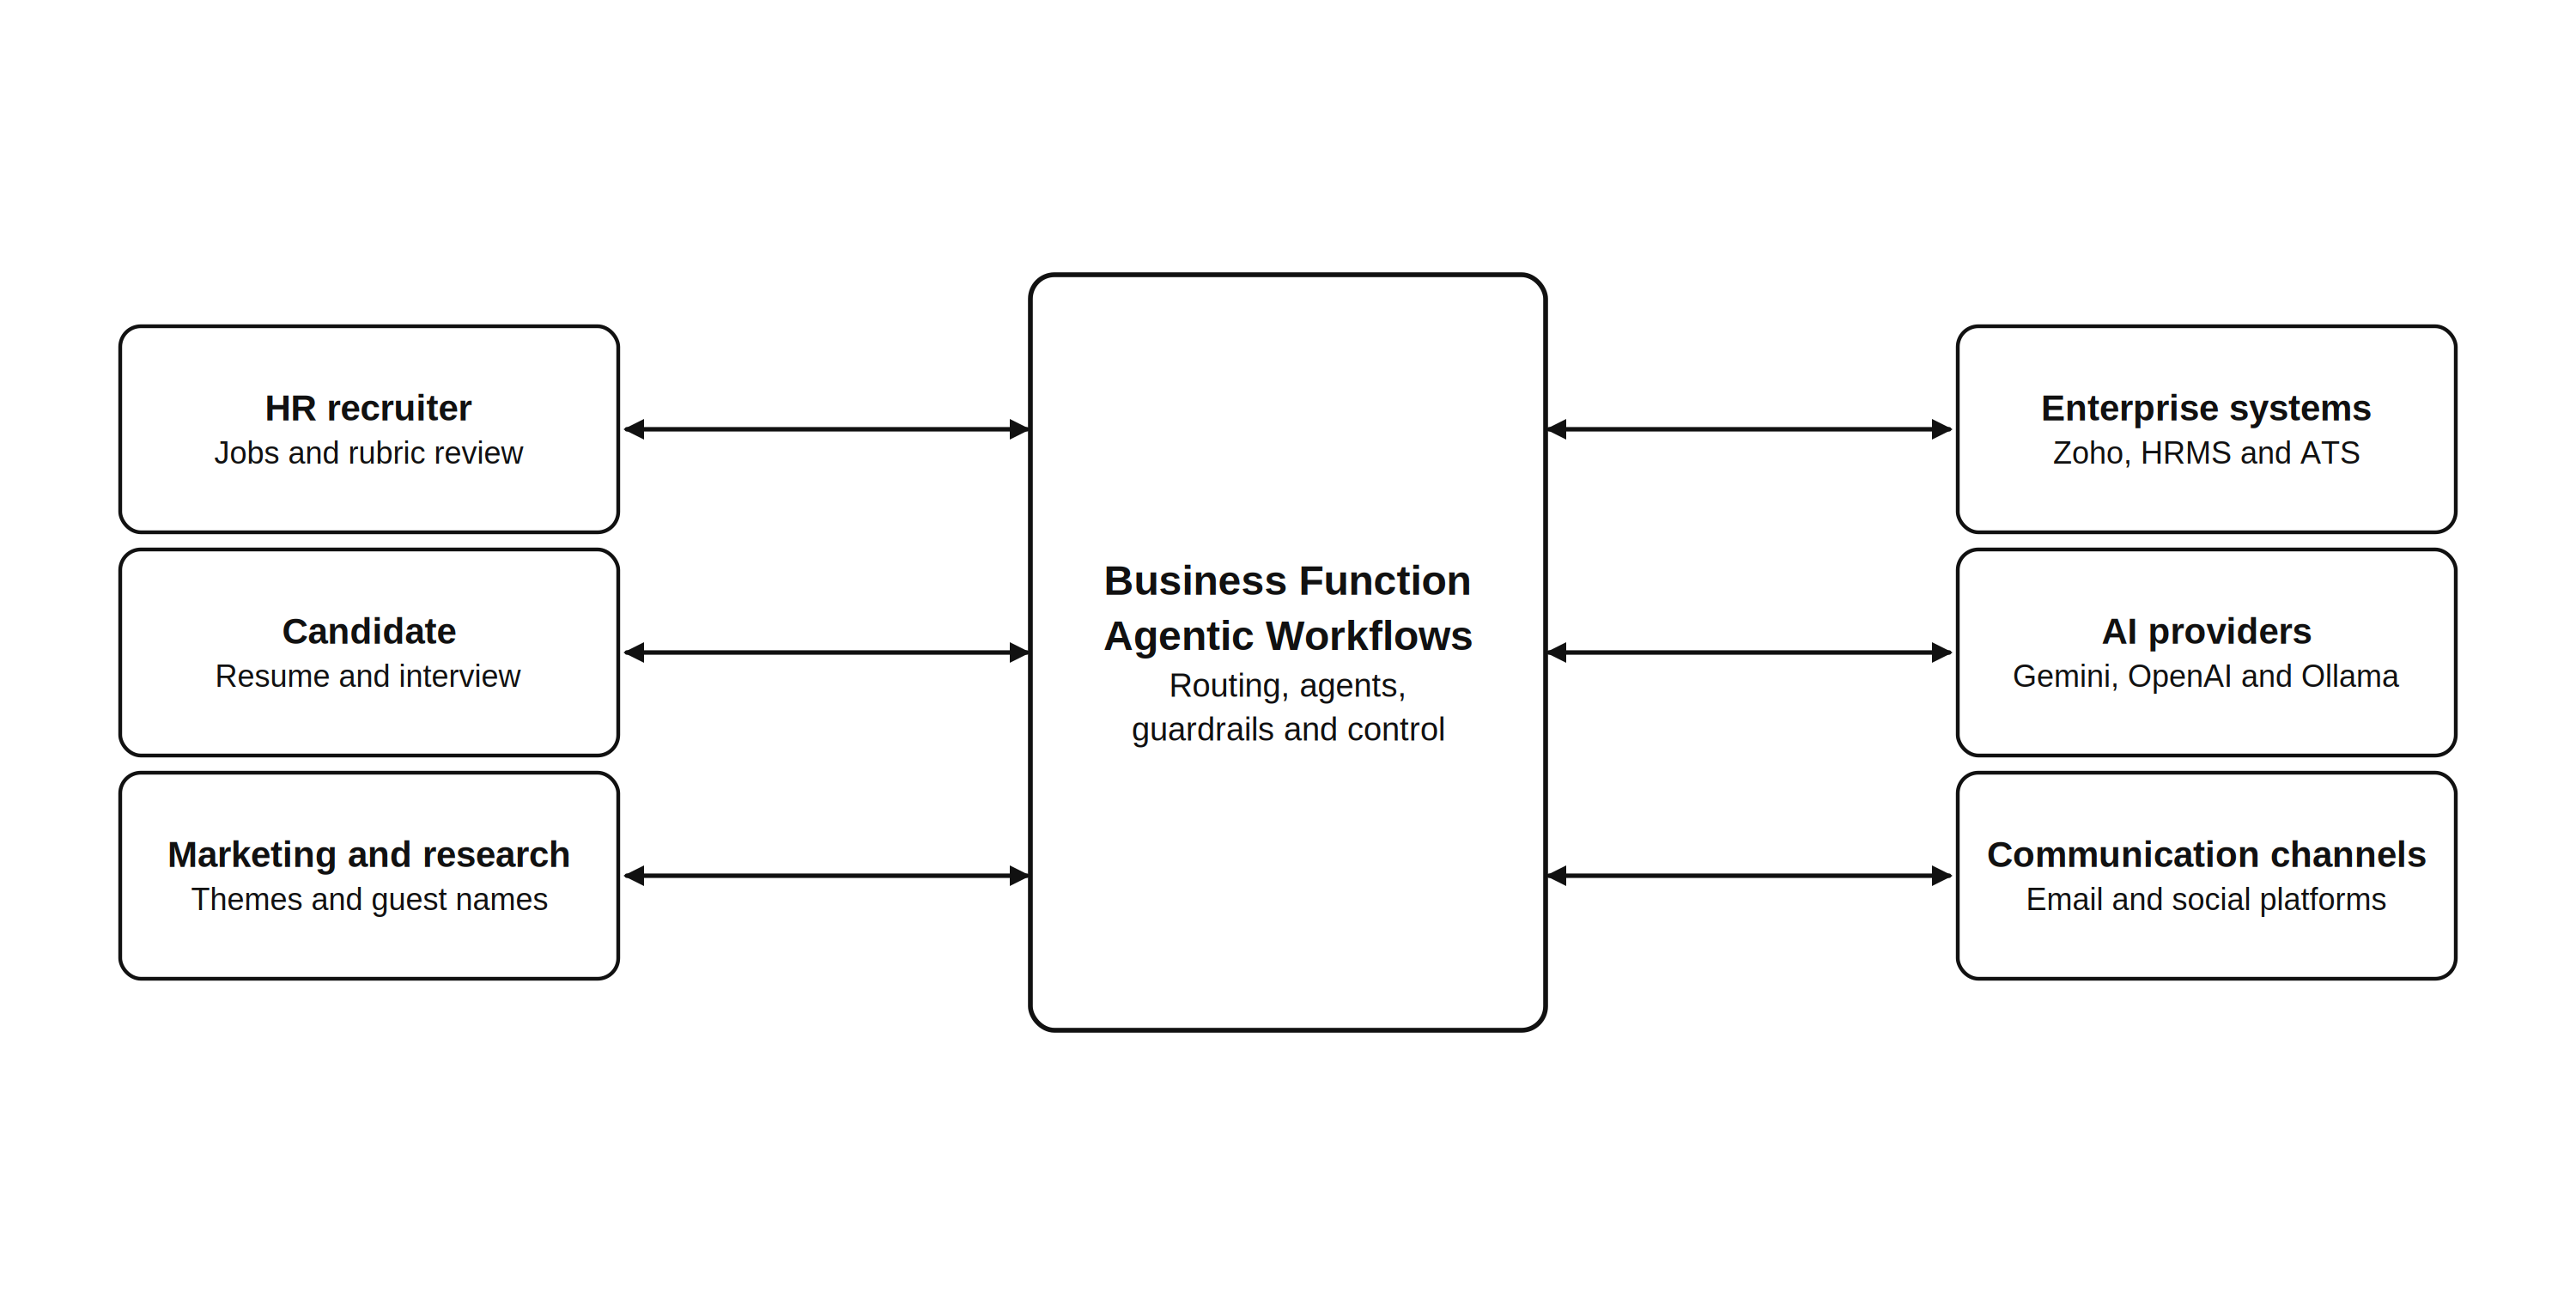
\includegraphics[width=\textwidth]{images/diagrams/fig_4_1_1_dfd_level_0.png}
  \caption{\textbf{Figure 4.1.1 DFD Level 0 of the System}}
\end{bodyfigure}

\noindent This diagram shows the whole system as a single process, \textit{Business Function Agentic Workflows}, which handles routing, agents, guardrails and control \cite{autogen,guo}. On the left are the HR recruiter, the candidate, and the marketing and research team, who supply jobs, resumes, interview responses, themes and guest names. On the right are the enterprise systems (Zoho, HRMS and ATS), the AI providers (Gemini, OpenAI and Ollama) and the communication channels, which exchange data with the system in both directions.

\vspace{14pt}

\begin{bodyfigure}[H]
  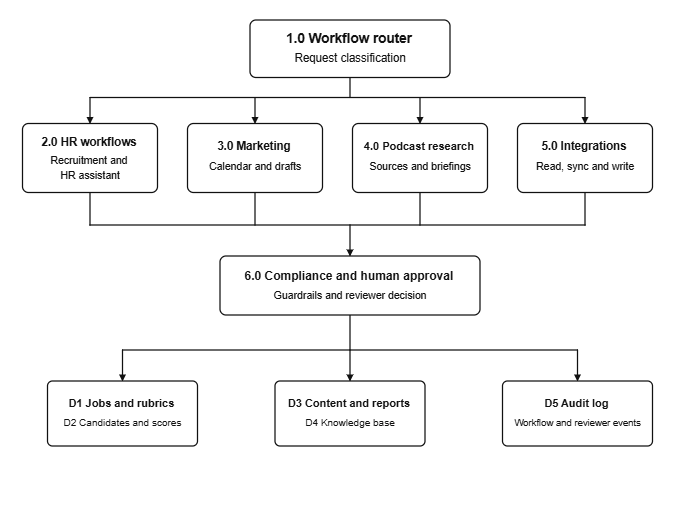
\includegraphics[width=\textwidth]{images/diagrams/fig_4_1_2_dfd_level_1.png}
  \caption{\textbf{Figure 4.1.2 DFD Level 1 of the System}}
\end{bodyfigure}

\noindent This diagram breaks the main process into six sub-processes: workflow router, HR workflows, marketing, podcast research, integrations, and compliance with human approval \cite{react,gan}. The router classifies each request and sends it to the matching workflow, and the outputs pass through the compliance and approval stage. Five data stores (jobs and rubrics, candidates and scores, content and reports, knowledge base, and audit log) hold the data these processes use and produce.

\clearpage
\subsection{UI/UX Diagram}

\begin{bodyfigure}[H]
  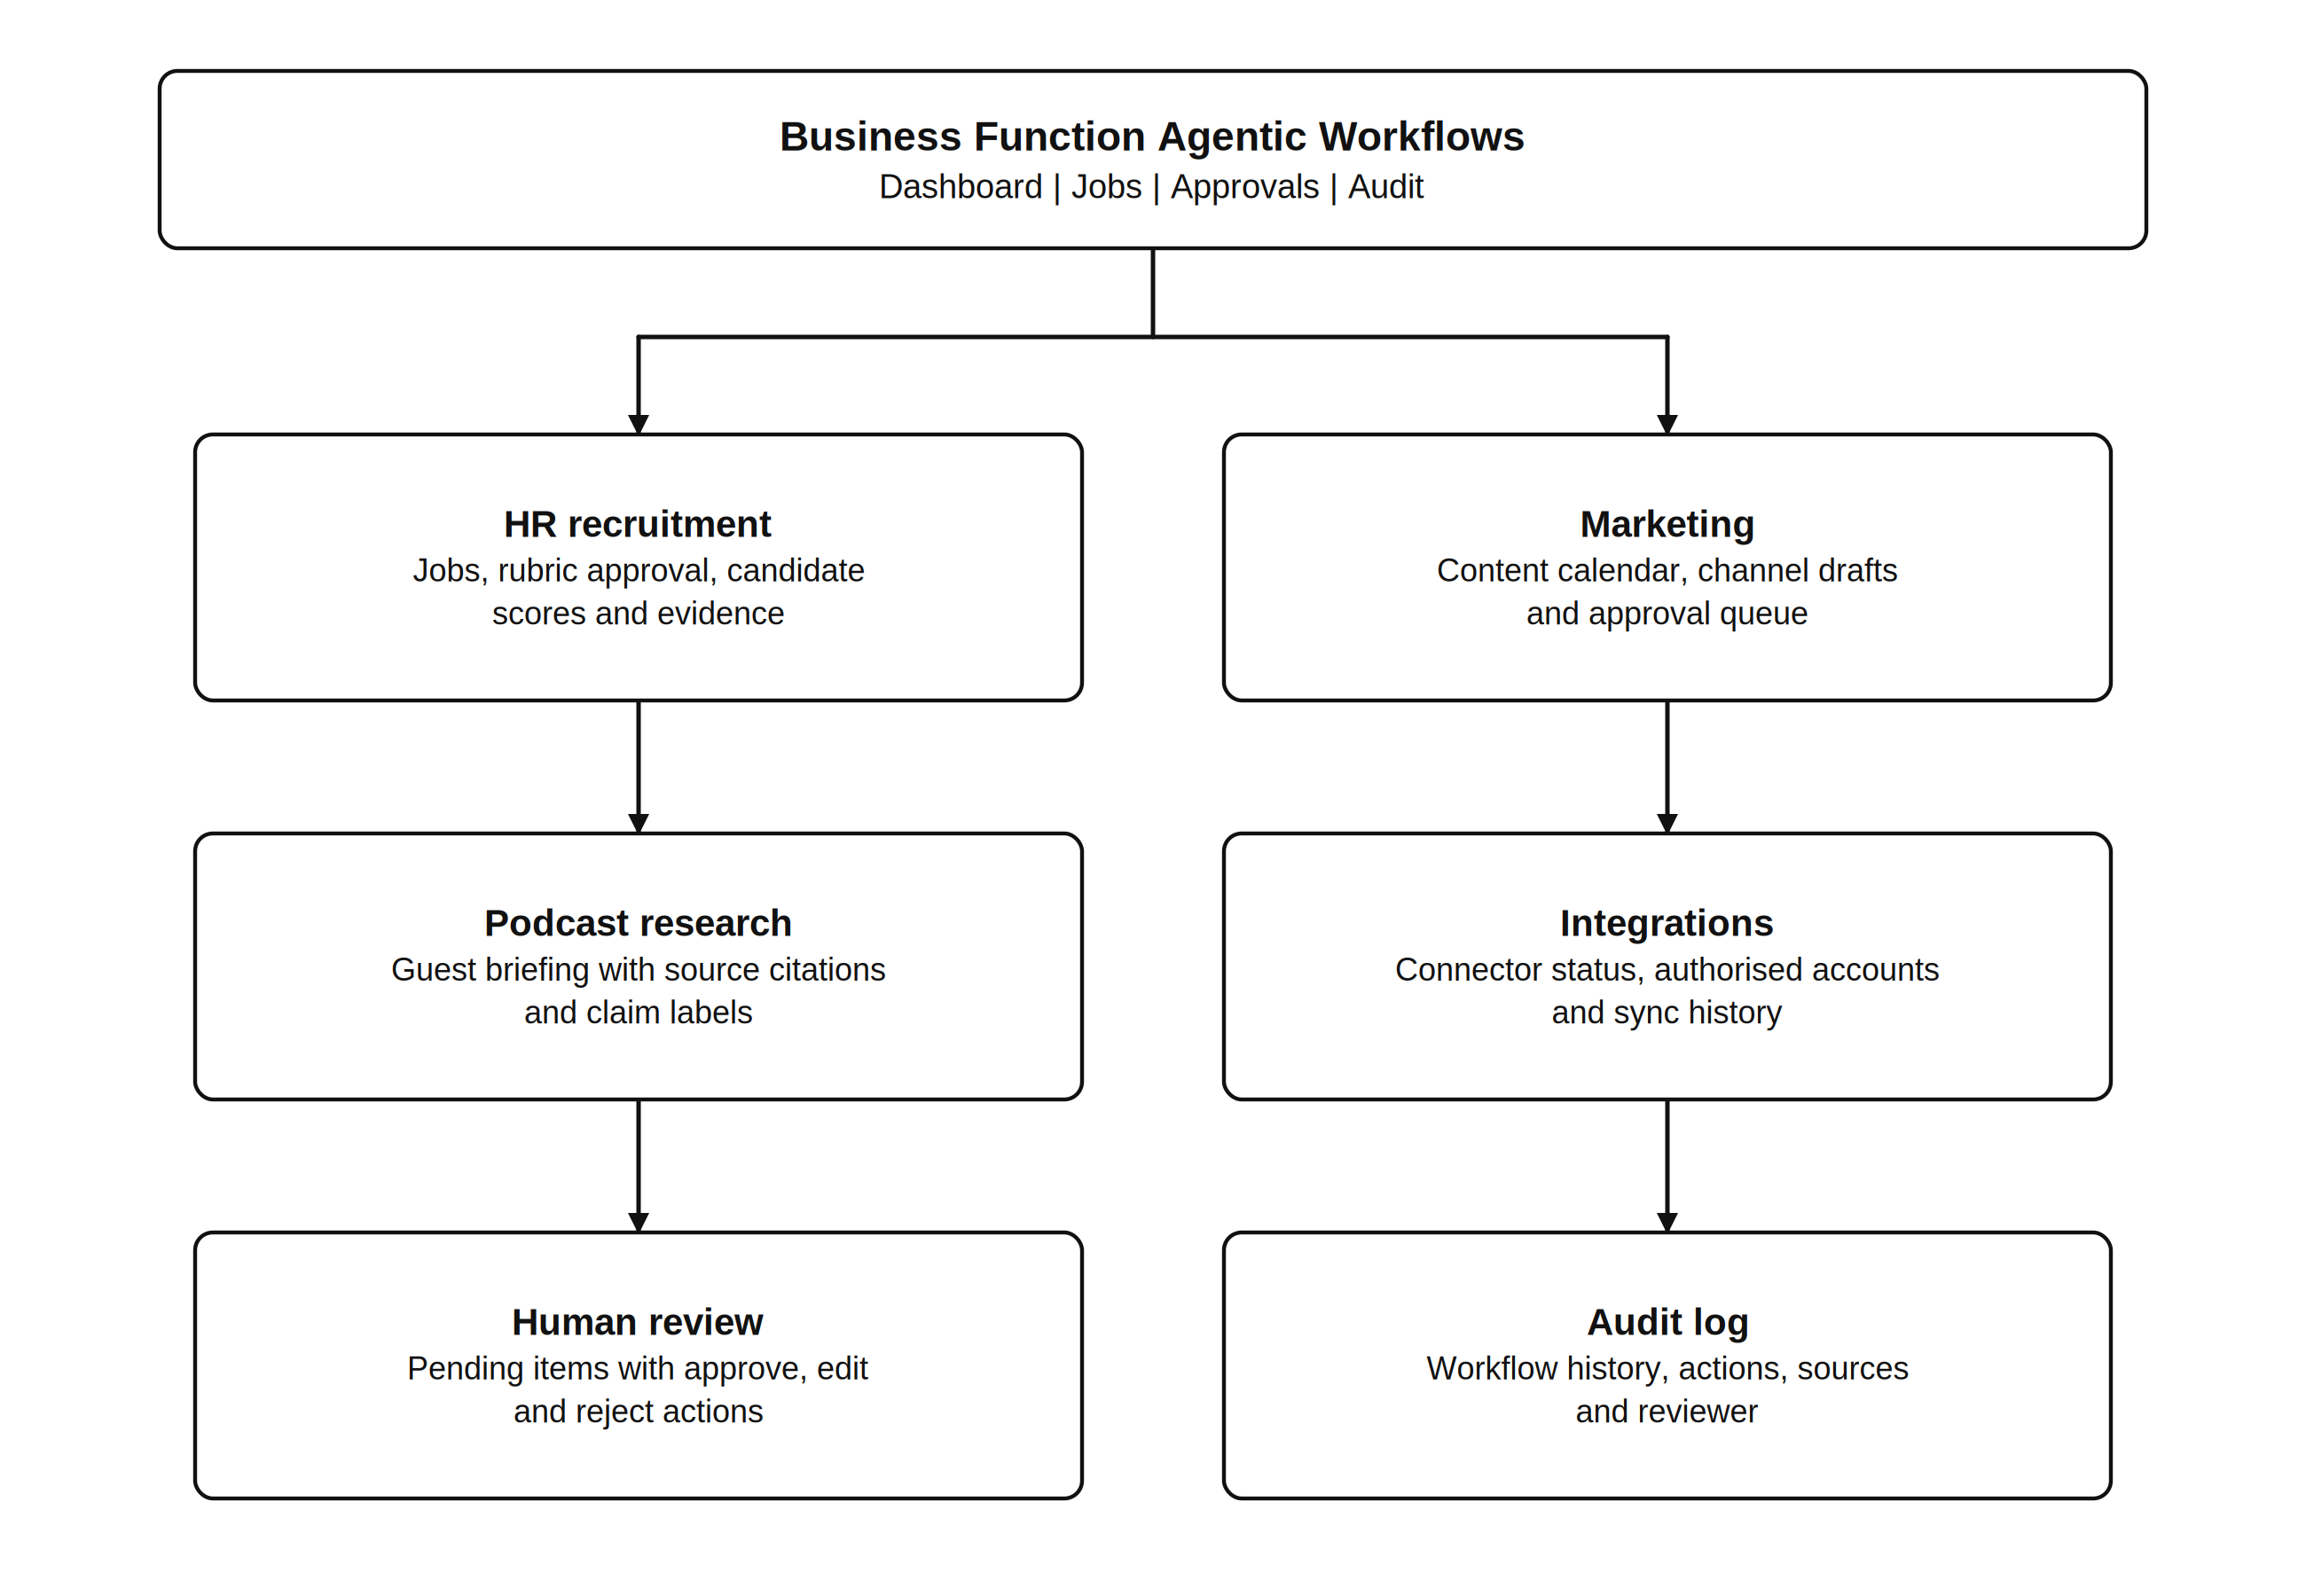
\includegraphics[width=\textwidth]{images/diagrams/fig_4_2_1_ui_ux_diagram.png}
  \caption{\textbf{Figure 4.2.1 UI/UX Diagram of the System}}
\end{bodyfigure}

\noindent This diagram shows the layout of the web application, with a main navigation bar for Dashboard, Jobs, Approvals and Audit. Below it are six functional screens: HR recruitment, marketing, podcast research, integrations, human review and audit log. Each screen shows the key information its users need, such as rubric approval and candidate scores, the content calendar and approval queue, cited briefings, connector status, and approve, edit and reject actions \cite{stuart,marketingfm}.

\clearpage
\subsection{Block Diagram}

\begin{bodyfigure}[H]
  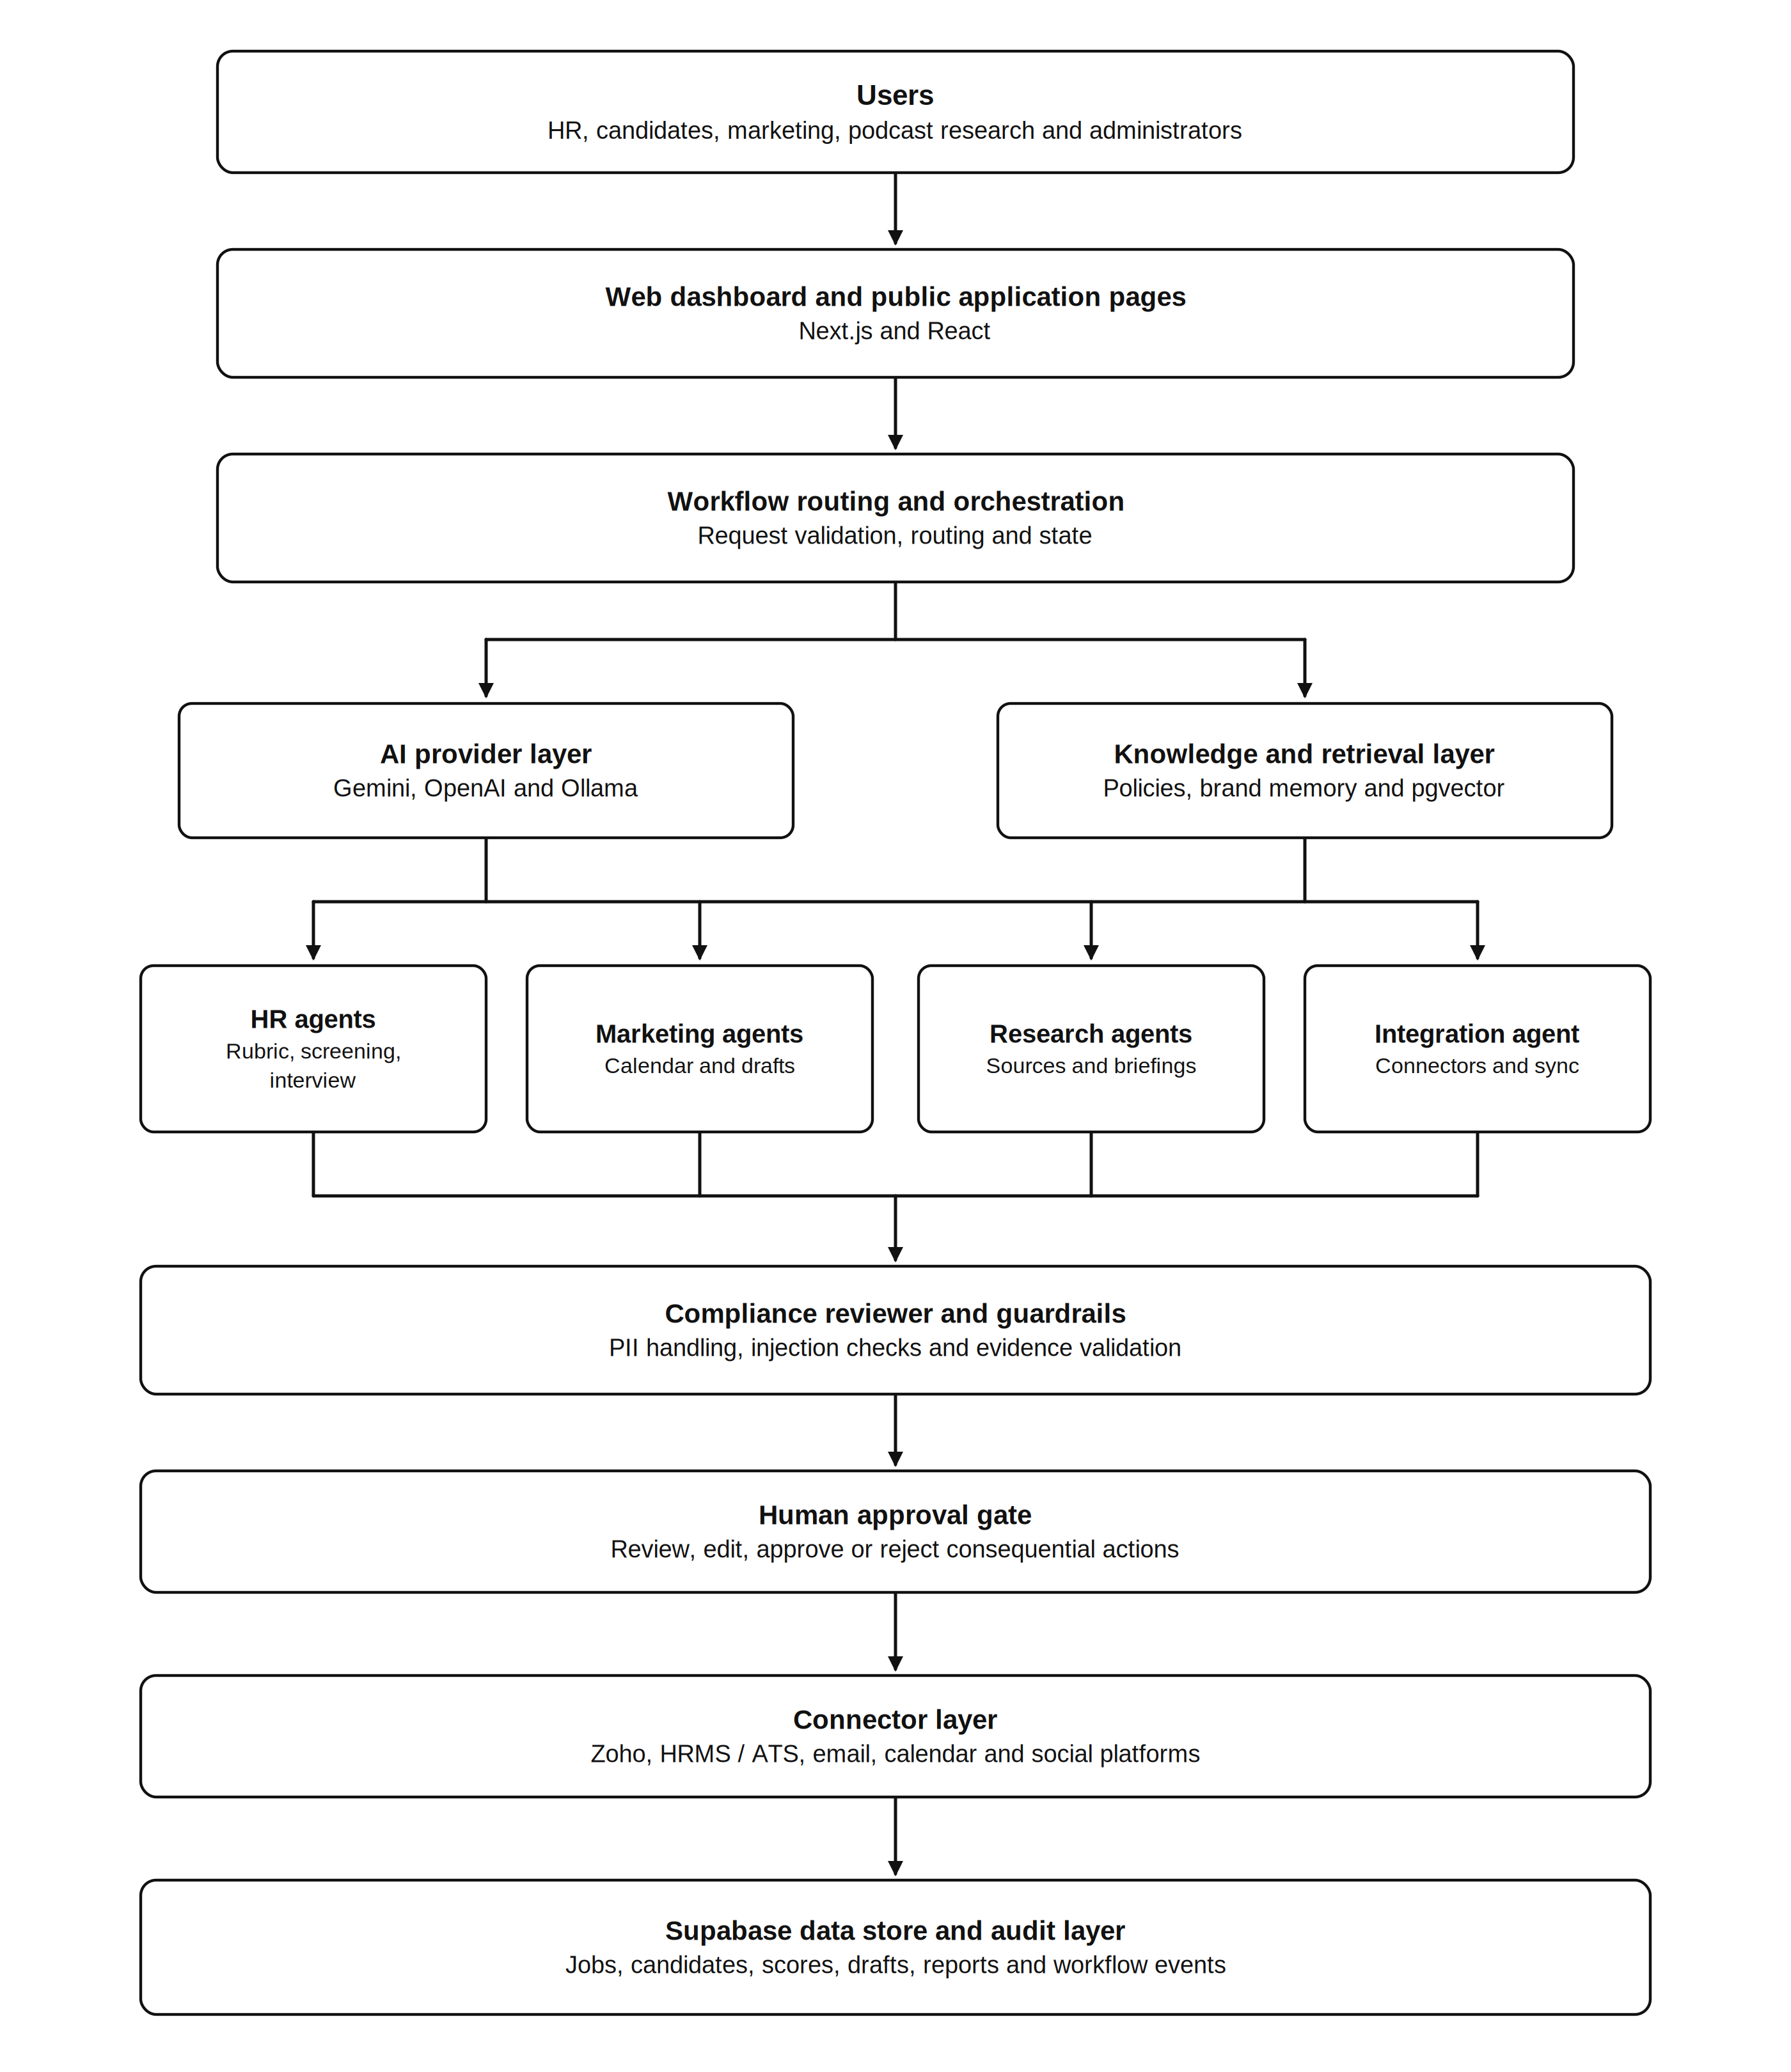
\includegraphics[width=\textwidth]{images/diagrams/fig_4_2_2_block_diagram.png}
  \caption{\textbf{Figure 4.2.2 Block Diagram of the System}}
\end{bodyfigure}

\noindent This diagram presents the layered architecture, from users and the Next.js and React dashboard down to workflow routing and orchestration. The AI provider layer and the knowledge and retrieval layer (policies, brand memory and pgvector) support the HR, marketing, research and integration agents. Outputs then pass through the compliance reviewer and guardrails, the human approval gate and the connector layer.

\clearpage
\subsection{Agent Workflow Diagrams}

\begin{bodyfigure}[H]
  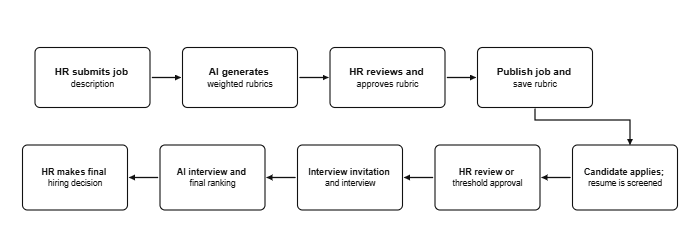
\includegraphics[width=\textwidth]{images/diagrams/fig_4_2_3_1_hr_agent_workflow.png}
  \caption{\textbf{Figure 4.2.3.1 HR Agent Workflow of the System}}
\end{bodyfigure}

\noindent The HR submits a job description, the AI generates weighted rubrics, and the HR reviews and approves them before the job is published and the rubric saved \cite{gan,stuart}. A candidate then applies and the resume is screened against the approved rubric. Depending on the result, the candidate goes through HR review or threshold approval, an interview invitation and an AI interview with final ranking, and the HR makes the final hiring decision.

\vspace{14pt}

\begin{bodyfigure}[H]
  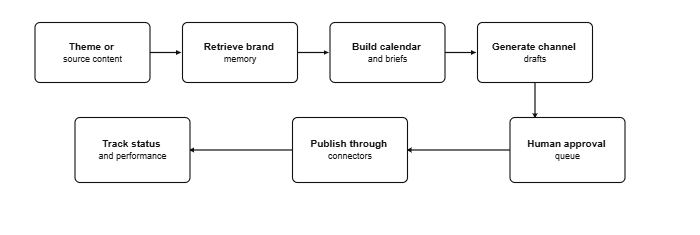
\includegraphics[width=\textwidth]{images/diagrams/fig_4_2_3_2_marketing_agent_workflow.png}
  \caption{\textbf{Figure 4.2.3.2 Marketing Agent Workflow of the System}}
\end{bodyfigure}

\noindent The workflow starts with a theme or source content, and the system retrieves brand memory to keep the output consistent with the organisation's voice \cite{marketingfm}. It then builds a content calendar and briefs and generates channel-specific drafts. The drafts go to a human approval queue before they are published through connectors, after which status and performance are tracked.

\clearpage

\begin{bodyfigure}[H]
  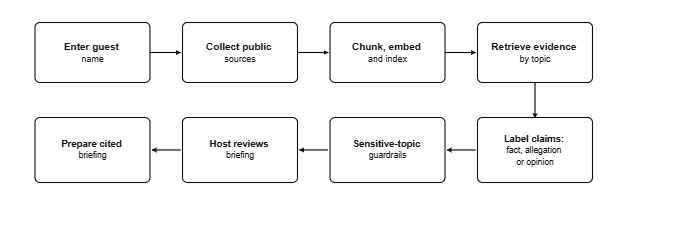
\includegraphics[width=\textwidth]{images/diagrams/fig_4_2_3_3_podcast_research_workflow.png}
  \caption{\textbf{Figure 4.2.3.3 Podcast Research Workflow of the System}}
\end{bodyfigure}

\noindent The user enters a guest name, and the system collects public sources, then chunks, embeds and indexes them for retrieval \cite{selfrag,cove}. It retrieves evidence by topic and labels each claim as fact, allegation or opinion, with sensitive-topic guardrails applied. A cited briefing is prepared for the host to review before the interview.

\vspace{14pt}

\begin{bodyfigure}[H]
  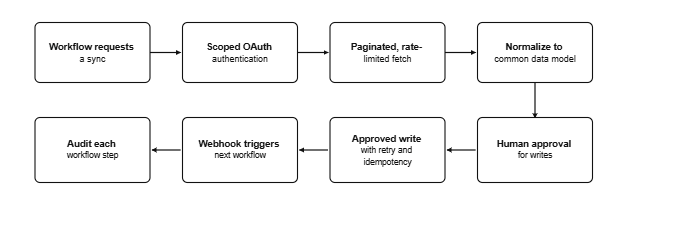
\includegraphics[width=\textwidth]{images/diagrams/fig_4_2_3_4_enterprise_integration_workflow.png}
  \caption{\textbf{Figure 4.2.3.4 Enterprise Integration Workflow of the System}}
\end{bodyfigure}

\noindent A workflow requests a sync, which is authenticated through scoped OAuth, and data is fetched with pagination and rate limiting \cite{toolformer,gorilla}. The data is normalised into a common data model, each step is audited, and webhooks can trigger the next workflow. Any write back to an external system needs human approval and is performed with retry logic and idempotency.
